\chapter{Related Work}
\label{chap:related}
Because there already is related work on information storage systems
for robots, \refsec{sec:rw-robmems} presents systems with approaches
and goals similar to this thesis. In \refsec{sec:databases}, we compare
database technologies and implementations that were considered as
basis for the robot memory and explain our choice
for the document-oriented database MongoDB in
\refsec{sec:basis-representation}. \refsec{sec:mongodb-extensions}
then presents related work about extensions of MongoDB that are
similar to the extensions we add for the use of MongoDB in our robot
memory.

\section{Information Storage Systems for Robots}
\label{sec:rw-robmems}
Because a memory can be an important part of a robot, there already are
various implementations and designs for it. However, there are only
some sophisticated robot memories that are separated into an own
component and can be universally used by multiple other components,
such as planners and reasoners. These robot memories with similar
approaches and goals are presented here. We start with the knowledge
processing systems KnowRob in \refsec{sec:knowrob} and OpenRobots
Ontology in \refsec{sec:oro}. Afterwards we present the Generic Robot
Database based on MongoDB and Fawkes in \refsec{sec:mongo-logging},
and Open-EASE, a combination of KnowRob and the Generic Robot
Database, in \refsec{sec:openease}.

\subsection{KnowRob}
\label{sec:knowrob}
KnowRob is an open source knowledge processing system for
cognition-enabled robots~\cite{KnowRob,KnowRob-Representation}. It is
designed to store knowledge about the environment and 
relate it to common sense knowledge to understand vaguely described
tasks, such as "set the table". For representation and inference of
knowledge, KnowRob uses Description Logic and approaches of the
semantic web.  Each small piece of information is represented as a
\emph{Resource Description Framework (RDF) triple}, e.g., \texttt{rdf(robot,
holding, cup)}, that are composed of a subject, predicate, and
object. A set of these RDF triples in a network can compose
common sense knowledge based on the \emph{Web Ontology Language
  (OWL)}~\cite{owl}. It uses \emph{ontologies}, which can roughly be described as
directed graphs setting objects or classes of objects into
relation. The graph can be represented with multiple RDF triples,
where the subject and object are nodes and the predicate is a directed
edge from the subject to the object. In these ontologies, it is
possible to represent common sense knowledge, such as \texttt{'milk is-a
perishable'}, \texttt{'refrigerator storage-place-for perishable'}, and
\texttt{'refrigerator is-a box-container'}. Thus a robot asked to bring milk
could infer that the milk is stored in the refrigerator, which needs
to be opened first since it is a box-like container.

The implementation and interface of KnowRob is based on the logic
programming language Prolog, which makes representing RDF triples and
inference with ontologies intuitive.  To be able to interface with
perception, KnowRob uses a concept called \emph{virtual knowledge
  base}. It allows computing needed information on demand instead of
storing everything providently. Thus special queries can be forwarded
to other components that compute the answer efficiently.  Especially
for perception based on sensor data or transformation of spatial
relations, this is advantageous compared to computing and storing all
possibly needed results in the memory.  KnowRob implements it with
Prolog predicates called \emph{Computables} which call C++ functions
of other components. This indeed slows down the computation of a query
but is more efficient than continuously computing and storing the
results or implementing and computing other components algorithms in
Prolog.  The concept inspired the usage of computables in this thesis.

To understand the robots environment, large and detailed ontologies
are necessary. KnowRob features acquiring and connecting these from
various sources, such as online common sense databases, the
cloud-based robot infrastructure RoboEarth~\cite{roboearth} and
websites for deriving object information from internet shops and
action recipes from how-to websites giving step by step instructions.
However, it has been found that this acquired knowledge needs a lot of
manual extension and verification before it can be used by the
robot~\cite{KnowRob-Web}. Encyclopedic knowledge often lacks action
information needed by the robot, e.g., how to grab tools, and
action recipes require human text understanding.
Furthermore large ontologies limit the performance of KnowRob because
of the Prolog implementation and general complexity. In contrast to
the robot memory of this thesis, KnowRob focuses on common
sense reasoning instead of an efficient and flexible on-line
back-end. It does not support sharing knowledge between multiple
robots and has a too strong focus on data only usable for reasoning
components. Although it can also represent spatio-temporal knowledge,
we have performance and scalability concerns with Prolog handling
larger data-sets, e.g., for storing locations of found object over long
time to learn the distribution where they can be found. Although
KnowRob can load ontologies from a hard drive, the memory acquired
during run-time is not persistently stored.

\subsection{OpenRobots Ontology (ORO)}
\label{sec:oro}
The OpenRobots Ontology (ORO) is an open source knowledge processing
framework for robotics~\cite{Oro}. It is designed to enable
human-robot interaction by featuring common sense ontologies similar to
KnowRob and modeling the human point of view. It also uses RDF triples
and OWL ontologies.  The triple storage is implemented in Jena, a Java
toolkit for RDF, and the inference with Pellet, a Java OWL
reasoner. Besides knowledge storing, querying and reasoning, ORO
features a modular architecture between the back-end storage and front
end socket server for querying. These modules add features such as
events that notify external components about changes, e.g., when
instances of certain classes are added or modified.
Another module adds representations of alternative perspectives that
should allow understanding the point of view of other agents.
For example when a human asks a robot to bring a
cup, there are two cups on a table and the robot should infer which
cup is meant by knowing that the other cup is occluded from the human's
point of view. Furthermore ORO features categorization to find
differences between objects, e.g., to ask if the blue cup or the red
cup was meant in a vague task description, and memory profiles for
distinguishing long-term knowledge and short-term knowledge that is
removed when the lifetime of a fact expires. Although these are useful
features and we realized the concepts of events and memory
profiles in this thesis, we do not use ORO as a basis. Due to its
focus on human-robot interaction and common sense reasoning, it is not
suitable for representing large amounts of data for non-reasoning
components because all data would have to be stored in RDF triples and
processed by the OWL reasoner. Furthermore, it does neither support
synchronizing a part of the knowledge with other robots nor knowledge
computation on demand.

\subsection{Generic Robot Database with MongoDB}
\label{sec:mongo-logging}
There already is a generic robot database developed with MongoDB as
data storage~\cite{RoboDB}. It is used to log data of the robot
middlewares Fawkes and ROS, and allows fault analysis and performance
evaluation. To achieve this, it taps into the messaging infrastructure
in ROS and the blackboard interfaces in Fawkes to store the data one
to one utilizing the flexibility of MongoDB being schema
free. Logged data can later be queried by the robot or a
developer. This allows better evaluation and fault analysis because
the data would otherwise be disposed and logging all kinds of data enables
retracing errors to find the source by setting it in relation to the 
Data-Information-Knowledge hierarchy~\cite{DIKW}. This work already
implements a basic connection to MongoDB in Fawkes for storing
documents and executing queries, which is used and extended in
this thesis. It also shows that MongoDB is a good choice because it
can handle querying a large database and writing a lot of data
efficiently while being flexible regarding how and which kind of data
is being represented.  However this work lacks some important concepts
needed for a robot memory as intended in this thesis. It is intended
as logging facility and not as working memory holding a world model
for multiple planners and reasoners. Therefore updating and querying
mechanisms for planners and reasoners are missing as well as triggers,
on demand computation, multi-robot synchronization, a
suitable front-end, and integration into knowledge-based systems.

\subsection{Open-EASE}
\label{sec:openease}
Open-EASE is a knowledge processing service for robots and AI
researchers~\cite{OpenEASE}. It is based on a combination of
KnowRob~\cite{KnowRob} and the Generic Robot Database with MongoDB in
ROS~\cite{RoboDB}. It is designed as a web service accessible by
robots via a socket connection and by humans via a web browser. It
uses KnowRob for common sense reasoning and storing the world model of
a robot. The Generic Robot Database is used to log data about robots
or humans performing manipulation tasks. This data can then be
accessed by using the virtual knowledge base concept to learn from
human demonstration and analyze faults. The focus of Open-EASE also is
on providing the recorded data and access to KnowRob to humans using
the web interface. This allows using Open-EASE as eLearning tool for
students, who can explore and experiment with the data and the robotic
system. Furthermore it fosters reproducing experiment results, e.g.,
for reviews, and visualizing them. Although the system is
accessible from multiple users and robots, which can query the same
Open-EASE instance, it is focused on single robot data and
non-collaborative processes because each user operates in his private
container with an individual knowledge base. This makes sense in the
context of student exercises, but is not suitable for multi-robot
systems or multiple knowledge-based systems sharing knowledge. If the
system is also usable or being extended for cooperating robots or
planners exchanging knowledge over the web service is not mentioned in
current publications or on the project
website\footnote{\url{http://www.open-ease.org/}}.

\todo[inline]{Section for ROSPlan/MongoStore?}

\section{Databases}
\label{sec:databases}
Since storing, keeping, and retrieving information with the robot
memory are central tasks of this thesis, the choice of a database
system is important. In the following, we present the three popular
database technologies, namely relational, graph-based, and
document-oriented databases. Because we later decide to use
document-orientation in robot memory, we conmpare document-oriented
databases in \refsec{sec:documentdbs}. MongoDB, the database
implementation used as a basis in this thesis, is presented separately
in \refsec{sec:mongodb}.

\subsection{Database Technologies}
\label{sec:db-designs}
There are multiple database technologies, which determine how data is
represented and structured. Thus they require different algorithms for
storing and querying and lead to different properties, such as
run-time, flexibility, scalability, and crosslinkability.

\subsubsection{Relational}
\label{sec:relational}
\emph{Relational databases} are a classic and broadly used database
technology for highly structured data. They are based on the
\emph{relational model}, introduced by
Codd~\cite{database-designs,relational}. The relational model
structures data into \emph{relations}, which can be described as
tables with attributes as columns and data entries as rows.
\begin{table}[ht]
  \begin{minipage}[b]{0.3\linewidth}\centering
  \begin{tabular}{ l|l|l }
    Id & Name & Age\\
    \hline
    A & Alice & 23\\
    B & Bob & 26\\
  \end{tabular}
  \\\vspace{0.2cm}
  (a) Relation Persons
\end{minipage}
\hspace{0.5cm}
\begin{minipage}[b]{0.3\linewidth}
\centering
  \begin{tabular}{ l|l }
    Id & Title\\
    \hline
    1 & Artificial Intelligence\\
    2 & Multi Agent Systems \\
  \end{tabular}
  \\\vspace{0.2cm}
  (b) Relation Books
\end{minipage}
\hspace{0.5cm}
\begin{minipage}[b]{0.3\linewidth}
\centering
  \begin{tabular}{ c|c }
    Person & Book\\
    \hline
    A & 1\\
    A & 2\\
  \end{tabular}
  \\\vspace{0.2cm}
  (c) Relation Borrowed
\end{minipage}
  \caption{Example for a relational database model about a
    library}
  \label{tab:relational-example}
\end{table}
\reftab{tab:relational-example} shows an example of a relational
database model of a library. Most relation contain a \emph{primary
  key}, a unique value to identify a row in the relation, e.g., the
\texttt{Id} columns in \reftab{tab:relational-example}. These keys
can be used as so-called \emph{foreign keys} to
link multiple relations, such as in
\reftab{tab:relational-example}(c). In which relations a database is
structured and which attributes relations contain is defined by the
\emph{schema} of the database.
\begin{wrapfigure}{r}{0.33\textwidth}
  \vspace{-0.4cm}
\begin{lstlisting}[style=SmallJSON,
  caption={SQL query},
  label=lst:sql,
  framexleftmargin=1pt, xleftmargin=0pt,
 morekeywords={}, numbers=none]
SELECT *
  FROM Borrowed
  JOIN Persons
    ON Borrowed.Person =
         Persons.Id
  JOIN Books
    ON Borrowed.Book = 
         Books.Id
\end{lstlisting}
\vspace{-8mm}
\end{wrapfigure}
To interact with a database management
system following the relational model, the \emph{Structured Query
  Language (SQL)} can be used. SQL is a formal language to insert,
update, and delete rows, change the database schema, and search the
database~\cite{database-def}. Queries can contain conditions for
attributes and group, sort, and aggregate results. An especially useful
feature of relational databases and SQL is joining multiple relations
by using foreign keys. For example, this allows listing the titles of
borrowed books together with the name of the borrower from
\reftab{tab:relational-example} with the query shown in \reflst{lst:sql}
\todo[inline]{check SQL query ...}
\todo[inline]{example relational database: PostgreSQL}

\subsubsection{Graph-Based}
\label{sec:graph-design}
\emph{Graph-based databases} model data structures as graphs with nodes and
edges~\cite{graphdbs}. Nodes usually represent entities and edges the
relations between them. Nodes and edges can have properties, such as a
name. This allows, for example, to model family trees with persons as
nodes, direct relation as edges, and names as properties of persons. In
comparison the to relational databases, there is no database schema
because the structure is intrinsically defined by the contained
data. Thus graph-based databases are called \emph{schema-free}. They
are well suited for domains with transitive relations, such as \texttt{'is
related to'}, and other problems that can be reduced to graph theory
problems, such as connectivity, because algorithms from graph theory
can directly operate on the graph. Therefore costly join operations, which
would be necessary in relational databases, can be
avoided~\cite{graphcomparison}. A graph-based data model that is
widely used in robotics is the \emph{Resource Description Framework
  (RDF)}~\cite{KnowRob-Representation,Oro,OpenEASE}. It represents
information as triples, e.g., \texttt{rdf(robot, holding, cup)}, that are
composed of a subject, predicate, and object~\cite{rdf}. Subjects and
objects are represented by nodes and predicates by edges. The query
language for RDF databases that is proposed as standard by the World
Wide Web Consortium is \emph{SPARQL}~\cite{sparql}. It provides operations that are
similar to SQL extended by graph traversal features.

\subsubsection{Document-oriented}
\label{sec:documene-design}
\emph{Document-oriented databases} store entities called \emph{documents},
which consist of key-value
pairs~\cite{mongodb,document-comparison,document-description}. In
contrast to relational databases, they are schema-free. Thus there is
no predefined schema that enforces the structure of
documents. Documents with similar structure are usually
grouped into \emph{collections}. Values can be accessed
by their key and can have different types, such as strings, numbers,
complex objects, such as dates and nested sub-documents. Therefore the documents
inserted in a collection implicitly define the structure during
run-time. This allows a flexible use of the database because
applications are not limited to a fixed schema and can, for example,
add key-value pairs during run-time when additional information needs
to be stored. Furthermore this simplifies software development, in which the
document structure tends to change often. Even if there are documents
with different structure, the application can choose to retrieve only
certain documents by giving a specialized query. Each document also
contains a unique key, similar to a primary key in relational
databases.
In contrast to relational databases, which \emph{normalize}
information into multiple relations to minimize redundancy, document-oriented ones focus on
bundling related information in documents (\emph{denormalization}).
This simplifies horizontal scaling in distributed systems because required
information is available at one place.
The query languages of document-oriented databases are not
so standardized as of relational databases shown in
\refsec{sec:documentdbs}. However, most document-oriented databases
have the usage of the \emph{JavaScript Object Notation (JSON)} as input format
in common.
\begin{wrapfigure}{r}{0.33\textwidth}
  \vspace{-0.4cm}
\begin{lstlisting}[style=SmallJSON,
  caption={JSON document},
  label=lst:json,
  framexleftmargin=1pt, xleftmargin=0pt,
 morekeywords={}, numbers=none]
 {
   "key": "value",
   "subdocument":
     {"x":3, "y":1},
   "array":
     [{"n":0.1},{"n":2}]
}
\end{lstlisting}
\vspace{-8mm}
\end{wrapfigure}
An example of a JSON document is shown in \reffig{lst:json}.
JSON is a lightweight data-interchange format similar to
the \emph{Extensible Markup Language (XML)}~\cite{json}. It is human
readable and assembles objects with key-value pairs. Because these
objects can also be nested, they can represent documents. Compared to
XML, JSON is faster and more compact~\cite{json-comparison}. In the
following, we omitt quotation marks around JSON keys for more compact
presentation.


\subsection{Document-oriented Databases}
\label{sec:documentdbs}
There are multiple database managing systems, which are based on the
document oriented model and could be used in this thesis. Here, we
present three popular open source implementations that we
considered. CouchDB and ArangoDB are introduced in this Subsection an
MongoDB is covered in the next Subsection in more detail.

\subsubsection{CouchDB}
\label{sec:couchdb}
Apache CouchDB\footnote{\url{http://couchdb.apache.org/}} is an open source document-oriented database
software~\cite{CouchDB,document-comparison}.
It is written in the concurrency-oriented language Erlang and
uses the JSON format to store data. Queries in CouchDB are realized with
so called \emph{views}, which are based on JavaScript functions,
e.g., to specify constraints, aggregation, updates. The
\emph{Application programming interface (API)} of
CouchDB is based on the Hypertext Transfer Protocol (HTTP) and thus focused on web applications, but
interfaces for other languages, such as C++, also exist. What
separates CouchDB from comparable database systems is its
\emph{multiversion concurrency control}. In a distributed system,
CouchDB does not guarantee consistency. It provides a system called
Multi-Master Replication, which allows writing to all replication
instances.  Conflicts can be solved similar to a version control
system, thus multiple conflicting versions can be kept in parallel for
later revision. Because of the multiversion concurrency control,
CouchDB also support asynchronous replication. Thus it is possible to
write on two replication instances concurrently. On a multi-robot
system that would avoid idling times waiting for write access, but
introduces the problem of solving conflicts later.

\subsubsection{ArangoDB}
\label{sec:arangodb}
ArangoDB\footnote{\url{https://www.arangodb.com/}} is an open source database managing system. What sets it
apart from other database managing systems is that it combines document
oriented and graph-based models in a so called
\emph{multi-model}~\cite{arango-manual,arango}. It supports the JSON
format, but stores the data in a binary format called
VelocityPack. The API is based on HTTP. ArangoDB uses the
\emph{Arango Query Language (AQL)}, which is inspired by SQL and
extended by document and graph features that account for the dynamic
schema. Queries can be enhanced with JavaScript functions, e.g., for
access graph features. Also the interface focuses on JavaScript, but
a C++ driver exists as well. Similar to CouchDB, ArangoDB also
features multiversion concurrency control. For a robot memory,
ArangoDB would have the advantage that ontological knowledge could be
properly represented and queried since it has a graph structure.

\subsection{MongoDB}
\label{sec:mongodb}
MongoDB\footnote{\url{https://www.mongodb.com/}} is a
document-oriented database. It provides many useful
features, such as flexible data structures, aggregation, and
distribution over multiple machines, which would take a large effort
to implement manually. It has proven as powerful and scalable data
storage and is widely used~\cite{mongodb,RoboDB}. MongoDB uses the
JSON format, but internally stores and evaluates documents in the
\emph{Binary JSON (BSON)} format.
\begin{figure}
  \begin{minipage}{0.58\linewidth}
\begin{lstlisting}[style=SmallJSON,
  caption={MongoDB document representing\protect\\ the position of a robot},
  label=lst:mongo-document,
  framexleftmargin=2pt, xleftmargin=2pt,
 morekeywords={}, numbers=none]
 {
   type: "position",
   name: "robot1",
   translation: {x:2.5, y:1.0, z:0.0},
   rotation: {x:0.0, y:0.0, z:0.0, w:1.0},
   timestamp : ISODate("2016-05-19T15:26:34.466Z")
 }
\end{lstlisting}
  \end{minipage}
  \begin{minipage}{0.42\linewidth}
\begin{lstlisting}[style=SmallJSON,
  caption={MongoDB query yielding the document in \reflst{lst:mongo-document}},
  label=lst:mongo-query,
  framexleftmargin=2pt, xleftmargin=10pt,
 morekeywords={}, numbers=none]
db.positions.find(
  {
    type: "position",
    name: "robot1",
    timestamp : {"$gt":
      ISODate("2016-05-19T15:26:34.000Z")}
  })
\end{lstlisting} %$
  \end{minipage}
  \vspace{-0.8cm}
\end{figure}
\reflst{lst:mongo-document} shows such a document
used for storing the position of a robot.

Queries in MongoDB are similar to documents because the arguments of
query functions also use the document structure. An example query is shown
in \reflst{lst:mongo-query}. It searches for all documents in the
collection \texttt{positions} that have matching values for
\texttt{type} and \texttt{position}, and are up to date, thus with a
timestamp greater than the given one. Multiple key-value pairs in a
query are conjunctive.  Values can be checked and compared as in the
example with a variety of operators such as \texttt{not}, \texttt{or},
\texttt{equals}, \texttt{greater than}, etc. These queries can be
evaluated very quickly, especially when \emph{indexing} is
used. Indexing is a
database feature that, similary to binary search, allows to lookup
documents faster than in linear time by sorting them for combination of document
keys, the \emph{index}. For more complex queries, it is possible to add arbitrary
JavaScript functions, which check if documents are matched.
Furthermore, it is possible to aggregate
results using the \emph{Map-Reduce} paradigm~\cite{mapreduce}, which
maps resulting documents to intermediate documents which are then
reduced until the end-result is found. For example this allows
querying for the nearest visible object by getting all visible
objects, mapping their position to a distance and reducing them to the
nearest one by dropping more distant ones when comparing them.
\todo[inline]{explain map and reduce steps more?}
 The
higher expressiveness of these queries comes with the price of slower
computation. However, the computational effort can be reduced by
formulating queries smartly. Many usual queries,
e.g. \reflst{lst:mongo-query}, can be formulated without using
\texttt{where} operators. Furthermore, complex queries can be nested to
filter documents first with a fast query and execute the
computationally costly query only on the remaining documents.
\begin{wrapfigure}{r}{0.3\textwidth}
  \centering
  \vspace{-5mm}
  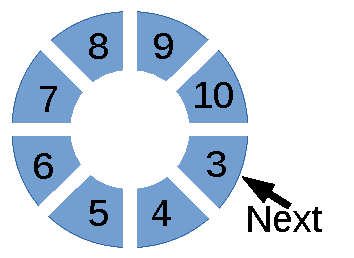
\includegraphics[width=0.3\textwidth]{draw/capped-collection}%
  \caption[Sketch of capped collection of size 8 after inserting the numbers 1-10 in
  this order]{Sketch of capped collection of size 8 after inserting the numbers 1-10 in
  this order}
  \vspace{-3mm}
  \label{fig:capped-collection}
\end{wrapfigure}
MongoDB also features fixed-size collections that are similar
to ring buffers. These are called \emph{capped collections} and order
documents by insertion order.
As \reffig{fig:capped-collection}
visualizes, new entries replace the oldest ones when the capped
collection is full.
An especially useful feature of MongoDB that allows sharing knowledge
between multiple robots is \emph{replication}. Replication is a
process that distributes a database onto multiple machines.  One
MongoDB instance called \emph{Primary} initially copies the database
to other instances called \emph{Secondaries}.  Afterwards, all
modifications to the primary database, which are stored in a separate,
capped collection called \emph{operations log (oplog)}, are forwarded to the
secondaries to keep them synchronized and consistent.  This is often
used in web-services to distribute read-queries and their computation
on multiple machines and to keep backups.  Read only queries can be
computed by Primary and Secondary instances. Modifying queries are
forwarded to the Primaries to guarantee consistency.  MongoDB can also
group multiple instances into a \emph{Replica Sets}, which
automatically manages the primary election when necessary. By using
replication, multiple robots can robustly share a common and
consistent world model. Robot specific knowledge can be kept in a
separate and not replicated database to avoid unneeded
communication. It is also possible to distribute write operations with
a technique called \emph{Sharding}. Sharding builds on Replica Sets
and splits the database into multiple \emph{shards}. Because each
shard can have its Primary on another machine, the write operations on
the database are distributed among the machines. This allows MongoDB
to scale in an application with too many writes for a single
machine.

\section{Why choose MongoDB as Basis of the Robot Memory?}
\label{sec:basis-representation}
In this section, we compare data storage systems that can be used as a
basis for the robot memory of this thesis and explain why we chose a
document-oriented database and MongoDB in particular. The possible
systems we compare are introduced in
the background and related work and are production systems,
ontologies, relational databases, and document-oriented databases.

One possibility for an underlying basis system is a production system
and CLIPS in particular. The information stored in the robot memory
can be represented by facts in the volatile fact base. In these facts,
key-value pairs can be used according to a predefined fact
template. The main advantage of a production system is its reasoning
capability that allows inferring more information and knowledge from
what is inserted and combining it with the existing fact base. For
example, this would allow inserting new observations and deriving an
updated world model, which can later be extracted. However,
this would be domain dependent because special rules for updating and inferring
would be required. Compared to other data storage systems,
CLIPS query features for access by external components are very
limited. For example, it would not scale for large data-sets due to the
lack of indexing. The rule matching capabilities of CLIPS are not
suitable for querying because each query would require a new rule that
changes the graph underlying the RETE algorithm and thus causes a
large computational overhead~\cite{Rete}.

Ontologies and RDF triples from the Web Ontology Language are another
possibility for a data storage system of the robot memory. Especially
KnowRob uses these and was considered as a basis for this
thesis. Information can be represented by RDF triples and embedded in
an ontology graph. The main advantage is, that this allows reasoning
while answering a query because the query can be reformulated using
backwards chaining with the ontology as a basis. A disadvantage of this is
the scalability with the sizes of the stored data and ontology. For
example, the robot memory should be able to store a large data-set
about object observations to learn their spatio-temporal
distribution. Furthermore, the information is not stored persistently
and can not be distributed in a multi robot system.

Compared to both previous approaches with ontologies and production
systems, database systems focus on data storage and querying instead
of reasoning. We think that they are a better basis for a robot memory
because they allow separating the concerns of storing and remembering
on the one hand, and reasoning, planning, and other robotic
applications on the other hand. They are designed to work as efficient
data storage with rich querying and distribution features. The
separation makes it possible for multiple systems to work with the
robot memory and to collaborate using the robot memory for information
exchange. When for example the common
sense reasoning of KnowRob should be integrated into a robot system,
the robot memory could store the required information in the database
and provide KnowRob with the required information and
ontologies. Furthermore, other systems such as a PDDL-based planner or a
component learning object distributions from observations can also use the
common basis in an efficient way. Before choosing a concrete database
managing system, we have to decide between a relational database and a
document-oriented database. Graph databases are not suited very well
because the information we want to represent often does not have a
graph structure, such as a world model of the RCLL or memorized object
observations. Thus the main advantages of graph databases, namely searching
and traversing a graph, are not so important. Relational databases provide powerful query features,
such as joining over multiple relations. Document-oriented databases
are schema free and thus allow a higher flexibility during development
and run-time. This flexibility is important because the representations of
information on the robot tend to change during development and it is
possible to group documents with similar purpose and different
attributes together, e.g., facts of a world model. Because of
denormalization, document-oriented databases avoid
joining over many relations by bundling information that
belongs together in a single document, e.g., with nesting. Especially this
allows document-oriented databases to scale horizontally and host a
distributed robot memory. These arguments lead to
the choice of a document-oriented database.

MongoDB is especially well suited for this thesis because of its
performance and scalability compared to the document-oriented
databases CouchDB and
ArangoDB~\cite{arango-vs-mongo}. Especially compared to
CouchDB, MongoDB provides faster interaction times~\cite{db-comparison}. This could be
caused by the HTTP interface or by the fact that queries in CouchDB purely rely on JavaScript
functions that have to be evaluated and computed during querying. The
query language of MongoDB also provides an additional syntax for
simple queries for faster evaluation in C++. Compared to ArangoDB,
MongoDB has a larger community and more features, such as Map-Reduce
and saving larger files. Furthermore it was already used successfully
and efficiently in Fawkes and the RCLL as logging
database~\cite{RoboDB,RCLL2015Eval}.

\section{MongoDB Extensions}
\label{sec:mongodb-extensions}
The work of this thesis uses MongoDB as a basis and extends it with
some concepts that are important for the usage in robot memory. In
this section, we present MongoDB extensions which are related to our
extensions, such as triggers for notifications about changes
in the database.

\subsection{Trigger}
\label{sec:mongodb-trigger}
In the database jargon, a trigger is a piece of code that is
automatically executed after a specified event, such as a change in
the database. Thus a trigger allows the user to react to events
without polling. Triggers are common in relational database management
systems, such as PostgreSQL~\cite{postgresql}. MongoDB does not
provide triggers, but there are multiple projects providing them as
extension~\cite{mongodb-trigger}. A simple way to realize
triggers on insertion events is using capped collections of MongoDB
because they order documents by the time of
insertion. The lazy and
iterative query evaluation strategy of MongoDB allows querying the
capped collection and keeping the cursor if there are no more
documents. After some time, the query can be continued from the
position of the cursor to check all documents that were inserted in the
meantime because they were just appended after the documents inserted
before. Conveniently MongoDB uses a capped collection to synchronize
changes in a Replica Set. This capped collection, called the
\emph{Oplog}, can also be queried by the user and allows listening to
changes in the Replica Set just as described above. In this thesis, we
also use the Oplog to implement trigger for the robot memory.

\subsection{Multi-Master Replication}
\label{sec:mongodb-multi-master}
There also exist an extensions of MongoDB which implement a
\emph{Multi-Master Replication}. It is called \emph{MongoDB
  MultiMaster (MMM)}\footnote{\url{https://github.com/rick446/mmm}}
and enables writing to each instance of a distributed MongoDB
database~\cite{mongodb-multi-master}. Changes can be immediately
applied locally and are synchronized later to the other
instances. This allows faster writing especially if the other
instances are not available for some time and would be advantageous in
the RCLL, where a crowded WiFi can lead to large latencies. However,
MMM is not focused on consistency and ignores write conflicts. Other
disadvantages are increased overall communication and database
size. This is caused by the implementation of MMM, which uses an usual
Master-Slave replication for each instance. Each instance consists of
one Master of these replications and Slaves for the other. MMM then
applies changes in a Slave replication to the local Master.  To detect
changes in a replica, MMM utilizes MongoDB's Oplog similar to this
thesis. It queries the Oplog, which is capped collection, as described
in the \refsec{sec:mongodb-trigger}.

% \todo[inline]{related work zu on demand computation in MongoDB: Ontology mediated queries}
